\documentclass[
  shownotes,
  xcolor={svgnames},
  hyperref={colorlinks,citecolor=DarkBlue,linkcolor=DarkRed,urlcolor=DarkBlue}
  , aspectratio=169]{beamer}
\usepackage{animate}
\usepackage{amsmath}
\usepackage{amsfonts}
\usepackage{amssymb}
\usepackage{pifont}
\usepackage{mathpazo}
%\usepackage{xcolor}
\usepackage{multimedia}
\usepackage{fancybox}
\usepackage[para]{threeparttable}
\usepackage{multirow}
\setcounter{MaxMatrixCols}{30}
\usepackage{subcaption}
\usepackage{graphicx}
\usepackage{lscape}
\usepackage[compatibility=false,font=small]{caption}
\usepackage{booktabs}
\usepackage{ragged2e}
\usepackage{chronosys}
\usepackage{appendixnumberbeamer}
\usepackage{animate}
\setbeamertemplate{caption}[numbered]
\usepackage{color}
%\usepackage{times}
\usepackage{tikz}
\usepackage{comment} %to comment
%% BibTeX settings
\usepackage{natbib}
\bibliographystyle{apalike}
\bibpunct{(}{)}{,}{a}{,}{,}
\setbeamertemplate{bibliography item}{[\theenumiv]}

% Defines columns for bespoke tables
\usepackage{array}
\newcolumntype{L}[1]{>{\raggedright\let\newline\\\arraybackslash\hspace{0pt}}m{#1}}
\newcolumntype{C}[1]{>{\centering\let\newline\\\arraybackslash\hspace{0pt}}m{#1}}
\newcolumntype{R}[1]{>{\raggedleft\let\newline\\\arraybackslash\hspace{0pt}}m{#1}}


\usepackage{xfrac}


\usepackage{multicol}
\setlength{\columnsep}{0.5cm}

% Theme and colors
\usetheme{Boadilla}

% I use steel blue and a custom color palette. This defines it.
\definecolor{andesred}{HTML}{af2433}

% Other options
\providecommand{\U}[1]{\protect\rule{.1in}{.1in}}
\usefonttheme{serif}
\setbeamertemplate{itemize items}[default]
\setbeamertemplate{enumerate items}[square]
\setbeamertemplate{section in toc}[circle]

\makeatletter

\definecolor{mybackground}{HTML}{82CAFA}
\definecolor{myforeground}{HTML}{0000A0}

\setbeamercolor{normal text}{fg=black,bg=white}
\setbeamercolor{alerted text}{fg=red}
\setbeamercolor{example text}{fg=black}

\setbeamercolor{background canvas}{fg=myforeground, bg=white}
\setbeamercolor{background}{fg=myforeground, bg=mybackground}

\setbeamercolor{palette primary}{fg=black, bg=gray!30!white}
\setbeamercolor{palette secondary}{fg=black, bg=gray!20!white}
\setbeamercolor{palette tertiary}{fg=white, bg=andesred}

\setbeamercolor{frametitle}{fg=andesred}
\setbeamercolor{title}{fg=andesred}
\setbeamercolor{block title}{fg=andesred}
\setbeamercolor{itemize item}{fg=andesred}
\setbeamercolor{itemize subitem}{fg=andesred}
\setbeamercolor{itemize subsubitem}{fg=andesred}
\setbeamercolor{enumerate item}{fg=andesred}
\setbeamercolor{item projected}{bg=gray!30!white,fg=andesred}
\setbeamercolor{enumerate subitem}{fg=andesred}
\setbeamercolor{section number projected}{bg=gray!30!white,fg=andesred}
\setbeamercolor{section in toc}{fg=andesred}
\setbeamercolor{caption name}{fg=andesred}
\setbeamercolor{button}{bg=gray!30!white,fg=andesred}


\usepackage{fancyvrb}
\newcommand{\VerbBar}{|}
\newcommand{\VERB}{\Verb[commandchars=\\\{\}]}
\DefineVerbatimEnvironment{Highlighting}{Verbatim}{commandchars=\\\{\}}
% Add ',fontsize=\small' for more characters per line
\usepackage{framed}
\definecolor{shadecolor}{RGB}{248,248,248}
\newenvironment{Shaded}{\begin{snugshade}}{\end{snugshade}}
\newcommand{\AlertTok}[1]{\textcolor[rgb]{0.94,0.16,0.16}{#1}}
\newcommand{\AnnotationTok}[1]{\textcolor[rgb]{0.56,0.35,0.01}{\textbf{\textit{#1}}}}
\newcommand{\AttributeTok}[1]{\textcolor[rgb]{0.77,0.63,0.00}{#1}}
\newcommand{\BaseNTok}[1]{\textcolor[rgb]{0.00,0.00,0.81}{#1}}
\newcommand{\BuiltInTok}[1]{#1}
\newcommand{\CharTok}[1]{\textcolor[rgb]{0.31,0.60,0.02}{#1}}
\newcommand{\CommentTok}[1]{\textcolor[rgb]{0.56,0.35,0.01}{\textit{#1}}}
\newcommand{\CommentVarTok}[1]{\textcolor[rgb]{0.56,0.35,0.01}{\textbf{\textit{#1}}}}
\newcommand{\ConstantTok}[1]{\textcolor[rgb]{0.00,0.00,0.00}{#1}}
\newcommand{\ControlFlowTok}[1]{\textcolor[rgb]{0.13,0.29,0.53}{\textbf{#1}}}
\newcommand{\DataTypeTok}[1]{\textcolor[rgb]{0.13,0.29,0.53}{#1}}
\newcommand{\DecValTok}[1]{\textcolor[rgb]{0.00,0.00,0.81}{#1}}
\newcommand{\DocumentationTok}[1]{\textcolor[rgb]{0.56,0.35,0.01}{\textbf{\textit{#1}}}}
\newcommand{\ErrorTok}[1]{\textcolor[rgb]{0.64,0.00,0.00}{\textbf{#1}}}
\newcommand{\ExtensionTok}[1]{#1}
\newcommand{\FloatTok}[1]{\textcolor[rgb]{0.00,0.00,0.81}{#1}}
\newcommand{\FunctionTok}[1]{\textcolor[rgb]{0.00,0.00,0.00}{#1}}
\newcommand{\ImportTok}[1]{#1}
\newcommand{\InformationTok}[1]{\textcolor[rgb]{0.56,0.35,0.01}{\textbf{\textit{#1}}}}
\newcommand{\KeywordTok}[1]{\textcolor[rgb]{0.13,0.29,0.53}{\textbf{#1}}}
\newcommand{\NormalTok}[1]{#1}
\newcommand{\OperatorTok}[1]{\textcolor[rgb]{0.81,0.36,0.00}{\textbf{#1}}}
\newcommand{\OtherTok}[1]{\textcolor[rgb]{0.56,0.35,0.01}{#1}}
\newcommand{\PreprocessorTok}[1]{\textcolor[rgb]{0.56,0.35,0.01}{\textit{#1}}}
\newcommand{\RegionMarkerTok}[1]{#1}
\newcommand{\SpecialCharTok}[1]{\textcolor[rgb]{0.00,0.00,0.00}{#1}}
\newcommand{\SpecialStringTok}[1]{\textcolor[rgb]{0.31,0.60,0.02}{#1}}
\newcommand{\StringTok}[1]{\textcolor[rgb]{0.31,0.60,0.02}{#1}}
\newcommand{\VariableTok}[1]{\textcolor[rgb]{0.00,0.00,0.00}{#1}}
\newcommand{\VerbatimStringTok}[1]{\textcolor[rgb]{0.31,0.60,0.02}{#1}}
\newcommand{\WarningTok}[1]{\textcolor[rgb]{0.56,0.35,0.01}{\textbf{\textit{#1}}}}
\usepackage{graphicx}
\makeatletter

\definecolor{airforceblue}{rgb}{0.36, 0.54, 0.66}

\usepackage{tikz}
% Tikz settings optimized for causal graphs.
\usetikzlibrary{shapes,decorations,arrows,calc,arrows.meta,fit,positioning}
\tikzset{
    -Latex,auto,node distance =1 cm and 1 cm,semithick,
    state/.style ={ellipse, draw, minimum width = 0.7 cm},
    point/.style = {circle, draw, inner sep=0.04cm,fill,node contents={}},
    bidirected/.style={Latex-Latex,dashed},
    el/.style = {inner sep=2pt, align=left, sloped}
}


\makeatother






%%%%%%%%%%%%%%% BEGINS DOCUMENT %%%%%%%%%%%%%%%%%%

\begin{document}

\title[Lecture 07]{Lecture 07: \\ Intro a Deep Learning, Redes Neuronales }
\subtitle{Aprendizaje y Minería de Datos para los Negocios}
\date{\today}

\author[Sarmiento-Barbieri]{Ignacio Sarmiento-Barbieri}
\institute[Uniandes]{Universidad de los Andes}


\begin{frame}[noframenumbering]
\maketitle
\end{frame}

%%%%%%%%%%%%%%%%%%%%%%%%%%%%%%%%%%%



%----------------------------------------------------------------------% 

\begin{frame}
\frametitle{Agenda}

\tableofcontents

\end{frame}
%----------------------------------------------------------------------%
\section{Recap}
%----------------------------------------------------------------------%

%----------------------------------------------------------------------%
\begin{frame}
\frametitle{Deep Learning: Intro}

\begin{itemize}
    \item Word Embedding surgen de las redes neuronales
    \medskip
  \item Redes neuronales son modelos simples
  \medskip
  \item Su fuerza reside en la simplicidad porque patrones básicos hacen que sean fácil de procesar y entrenar. 
  \medskip
  \item El modelo tiene combinaciones lineales que pasan a través de funciones no lineales de activación que se llaman nodos (o neuronas). 
  \medskip
  \item Un conjunto de nodos que toma diferente sumas ponderadas de los mismos insumos se llama capa (layer)
  \medskip
  \item  El resultado de los nodos de una capa se convierte en el insumo de la otra capa. 
\end{itemize}

\end{frame}

%----------------------------------------------------------------------%
\section{Deep Learning: Intro}
%----------------------------------------------------------------------%
\begin{frame}
\frametitle{Deep Learning: Recap}
  
  \begin{itemize}
    \item Empecemos con un modelo simple y familiar, el modelo lineal
  
  \end{itemize}

\def\layersep{2.5cm}

\begin{align}
y &= f(X) + u \\ \nonumber
y &= \beta_1 x_1 + \beta_2 x_2 + \beta_3 x_3  + u
\end{align}
\pause

\begin{figure}[H]
\centering

\begin{tikzpicture}[shorten >=1pt,->,draw=black!50, node distance=\layersep]
    \tikzstyle{every pin edge}=[<-,shorten <=1pt]
    \tikzstyle{neuron}=[circle,fill=black!25,minimum size=17pt,inner sep=0pt]
    \tikzstyle{input neuron}=[neuron, fill=green!50];
    \tikzstyle{output neuron}=[neuron, fill=red!50];
    \tikzstyle{annot} = [text width=4em, text centered]

    % Draw the input layer nodes
    \foreach \name / \y in {1,...,3}
    % This is the same as writing \foreach \name / \y in {1/1,2/2,3/3,4/4}
        \node[input neuron, pin=left:$x_\y$] (I-\name) at (0,-\y) {};

    % Draw the output layer node
    \node[output neuron,pin={[pin edge={->}]right:y}, right of=I-2] (O) {};

    % Connect every node in the input layer with every node in the
    % hidden layer.
    

    % Connect every node in the hidden layer with the output layer
    \foreach \source in {1,...,3}
        \path (I-\source) edge (O);

    \node[annot,above of=I-1, node distance=1cm] (i) {Input layer};
    \node[annot,right of=i] {Output layer};

\end{tikzpicture}
\end{figure}



\end{frame}
%----------------------------------------------------------------------%
\section{Multilayer Perceptrons}
%----------------------------------------------------------------------%
\begin{frame}
\frametitle{Multilayer Perceptrons}

\begin{itemize}
    \item Los modelos lineales pueden ser muy sencillos y perder la no linealidad que mejor aproximan $f^*(x)$
    \medskip
    \item Podemos superar estas limitaciones de los modelos lineales y manejar una clase de funciones más generales al incorporar una o más capas ocultas.
    \medskip
    \item Las redes feedforward, también llamadas redes neuronales de alimentación directa, o perceptrones multicapa (MLP), son los modelos de aprendizaje profundo por excelencia

\end{itemize}


\end{frame}

%----------------------------------------------------------------------%
\begin{frame}
\frametitle{Multilayer Perceptrons}

\begin{itemize}
\item Las redes neuronales feedforward son llamadas redes porque  generalmente se representan componiendo muchas funciones diferentes. 
\medskip
\item El modelo se asocia con un gráfico acíclico dirigido que describe cómo las funciones se componen juntas. Por ejemplo, podemos tener dos funciones $f^{(2)}$, $f^{(1)}$ y conectadas en una cadena para formar $f(x)=f^{(2)}(f^{(1)}(x))$ 
\medskip
 \item Estas estructuras de cadena son las estructuras de redes neuronales más utilizadas.
\end{itemize}
\end{frame}

%----------------------------------------------------------------------%
\begin{frame}
\frametitle{Multilayer Perceptrons}


\def\layersep{2.5cm}

\begin{figure}[H]
\centering
\begin{tikzpicture}[shorten >=1pt,->,draw=black!50, node distance=\layersep]
    \tikzstyle{every pin edge}=[<-,shorten <=1pt]
    \tikzstyle{neuron}=[circle,fill=black!25,minimum size=17pt,inner sep=0pt]
    \tikzstyle{input neuron}=[neuron, fill=green!50];
    \tikzstyle{output neuron}=[neuron, fill=red!50];
    \tikzstyle{hidden neuron}=[neuron, fill=blue!50];
    \tikzstyle{annot} = [text width=4em, text centered]

    % Draw the input layer nodes
    \foreach \name / \y in {1,...,4}
    % This is the same as writing \foreach \name / \y in {1/1,2/2,3/3,4/4}
        \node[input neuron, pin=left: $x_\y$] (I-\name) at (0,-\y) {};

    % Draw the hidden layer nodes
    \foreach \name / \y in {1,...,5}
        \path[yshift=0.5cm]
            node[hidden neuron] (H-\name) at (\layersep,-\y cm) {};

    % Draw the output layer node
    \node[output neuron,pin={[pin edge={->}]right:y}, right of=H-3] (O) {};

    % Connect every node in the input layer with every node in the
    % hidden layer.
    \foreach \source in {1,...,4}
        \foreach \dest in {1,...,5}
            \path (I-\source) edge (H-\dest);

    % Connect every node in the hidden layer with the output layer
    \foreach \source in {1,...,5}
        \path (H-\source) edge (O);

    % Annotate the layers
    \node[annot,above of=H-1, node distance=1cm] (hl) {Hidden layer};
    \node[annot,left of=hl] {Input layer};
    \node[annot,right of=hl] {Output layer};
\end{tikzpicture}
\end{figure}

\end{frame}
%----------------------------------------------------------------------%
\begin{frame}
\frametitle{Multilayer Perceptrons}


\begin{itemize}



\item La longitud total de la cadena le otorga la profundidad al modelo. El nombre “deep learning” surge de esta terminología. 
\medskip
\item La capa final de una red feedforward network se denomina
capa de salida
\medskip
\item Durante el entrenamiento de red neuronal, tratamos de entrenar $f(x)$ para estimar $f^*(x)$
\medskip
\end{itemize}

\end{frame}
%----------------------------------------------------------------------%
\begin{frame}
\frametitle{Multilayer Perceptrons}

\begin{itemize}

\item En el entrenamiento de datos observamos la primer capa, inputs ($x$), y la última capa, output ($y$)
\medskip
\item No observamos las capas intermedias, llamadas capas ocultas.
\medskip
\item Finalmente, estas redes son llamadas neuronales porque son inspiradas por
neurociencia.



\end{itemize}
\end{frame}

%----------------------------------------------------------------------%
\subsection{Worked Example}
%----------------------------------------------------------------------%
\begin{frame}
\frametitle{Worked Example: The "Exclusive OR (XOR)" Function}
\begin{itemize}
\item La disyunción exclusiva de un par de proposiciones, (p, q), supone que p o q es verdadero, pero no ambos
\item La tabla de la verdad es:

\begin{table}[H]
\begin{tabular}{lllll}
q  & p & q v p \\
\hline
0 & 0 & 0 \\
0 & 1 & 1 \\
1 & 0 & 1 \\
1 & 1 & 0 \\
\end{tabular}
\end{table}
\item Cuando exactamente uno de estos valores binarios es igual a 1, la función XOR 
regresa 1. De otra forma, regresa 0
\end{itemize}

\end{frame}
%----------------------------------------------------------------------%
\begin{frame}
\frametitle{Worked Example: The "Exclusive OR (XOR)" Function}

\begin{itemize}
\item Usemos un modelo lineal 

\begin{align}
y = X\beta + \iota \alpha 
\end{align}


 \begin{align}
 y=\left(\begin{array}{c}
0\\
1\\
1\\
0
\end{array}\right)X=\left(\begin{array}{cc}
0 & 0\\
0 &1\\
1 & 0\\
1 & 1
\end{array}\right)\iota=\left(\begin{array}{c}
1\\
1\\
1\\
1
\end{array}\right)
 \end{align}

\item Solución $ \alpha=\frac{1}{2} \,\,\,\beta=\left(\begin{array}{c}
0\\
0
\end{array}\right)
$


\item Predicción $\hat{y}=\left(\begin{array}{c}
\frac{1}{2}\\
\frac{1}{2}\\
\frac{1}{2}\\
\frac{1}{2}
\end{array}\right)$
\end{itemize}


\end{frame}
%----------------------------------------------------------------------%
\begin{frame}
\frametitle{Worked Example: The "Exclusive OR (XOR)" Function}

\begin{itemize}
 \item Usemos perceptroens multicapas (red feedforward) con una capa
oculta conteniendo dos unidades ocultas


\def\layersep{2cm}

\begin{figure}[H]
\centering
\begin{tikzpicture}[shorten >=1pt,->,draw=black!50, node distance=\layersep]
    \tikzstyle{every pin edge}=[<-,shorten <=1pt]
    \tikzstyle{neuron}=[circle,fill=black!25,minimum size=17pt,inner sep=0pt]
    \tikzstyle{input neuron}=[neuron, fill=green!50];
    \tikzstyle{output neuron}=[neuron, fill=red!50];
    \tikzstyle{hidden neuron}=[neuron, fill=blue!50];
    \tikzstyle{annot} = [text width=4em, text centered]

    % Draw the input layer nodes
    \foreach \name / \y in {1,...,2}
    % This is the same as writing \foreach \name / \y in {1/1,2/2,3/3,4/4}
        \node[input neuron, pin=left: $x_\y$] (I-\name) at (0,-\y) {};

    % Draw the hidden layer nodes
    \foreach \name / \y in {1,...,2}
        \path[yshift=0cm]
            node[hidden neuron] (H-\name) at (\layersep,-\y cm) {};

    % Draw the output layer node
    \node[output neuron,yshift=-0.5cm, pin={[pin edge={->}]right:y}, right of=H-1] (O) {};

    % Connect every node in the input layer with every node in the
    % hidden layer.
    \foreach \source in {1,...,2}
        \foreach \dest in {1,...,2}
            \path (I-\source) edge (H-\dest);

    % Connect every node in the hidden layer with the output layer
    \foreach \source in {1,...,2}
        \path (H-\source) edge (O);

    % Annotate the layers
    \node[annot,above of=H-1, node distance=1cm] (hl) {Hidden layer};
    \node[annot,left of=hl] {Input layer};
    \node[annot,right of=hl] {Output layer};
\end{tikzpicture}
\end{figure}
\footnotesize
\item Esta red tiene un vector de unidades ocultas $h$ que son calculadas por una
función $f^{(1)}(x;W , c)$. 
\item Los valores de estas unidades ocultas se utilizan luego como entrada para una segunda capa. \item La segunda capa es la capa de salida de la red. La capa de salida sigue siendo sólo un modelo de regresión lineal, pero ahora se aplica a $h$ en vez de a $x$
\item  La red ahora contiene dos funciones encadenadas juntas, $f(x;W , c, w, b) = f^{(2)}(f^{(1)}(x))$
\end{itemize}

\end{frame}
%----------------------------------------------------------------------%
\begin{frame}
\frametitle{Worked Example: The "Exclusive OR (XOR)" Function}

\begin{itemize}
    \item Qué $f^{(1)}$ deberíamos especificar?
    \medskip
    \begin{itemize}
    \item Claramente {\bf no} lineal, de lo contrario no tendria sentido la tarea
    \item Vamos a usar una unidad lineal rectificada o ReLU (usualmente la recomendación predeterminada, hay muchas otras!!)
    \item ReLU se define como $g(z)=max\{0,z\}$
    \end{itemize}
    
    \item Para $f^{(2)}$? Para este ejemplo, un modelo lineal será suficiente
    \medskip
    \begin{align}
    f^{(2)} = f^{(1)}w + b
    \end{align}
    \item Entonces, el modelo final es  
    \begin{align}
    f(x,W,C,w,b) = max\{0,XW+c\}\,w + b
    \end{align}
\end{itemize}

\end{frame}
%----------------------------------------------------------------------%
\begin{frame}
\frametitle{Worked Example: The "Exclusive OR (XOR)" Function}

\begin{itemize}
\item Suponga que esta es la solución al problema XOR  
\end{itemize}


\[
f(x)=max\{0,XW+c\}\,w+b
\]

\[
W=\left(\begin{array}{cc}
1 & 1\\
1 & 1
\end{array}\right)
\]

\[
c=\left(\begin{array}{cc}
0 & -1\\
0 & -1\\
0 & -1\\
0 & -1
\end{array}\right)
\]

\[
w=\left(\begin{array}{cc}
1 & -2\end{array}\right)
\]

 \[
 b = 0
 \]


\end{frame}
%----------------------------------------------------------------------%
\begin{frame}
\frametitle{Worked Example: The "Exclusive OR (XOR)" Function}

\begin{itemize}
\item Trabajemos el ejemplo paso a paso
\end{itemize}
\begin{align}
f(x)=max\{0,XW+c\}\,w+b
\end{align}

\[
XW=\left(\begin{array}{cc}
0 & 0\\
0 & 0\\
1 & 0\\
1 & 0
\end{array}\right)\left(\begin{array}{cc}
1 & 1\\
1 & 1
\end{array}\right)=\left(\begin{array}{cc}
0 & 0\\
1 & 1\\
1 & 1\\
2 & 2
\end{array}\right)
\]

\[
XW+c=\left(\begin{array}{cc}
0 & -1\\
1 & 0\\
1 & 0\\
2 & 1
\end{array}\right)
\]

\[
max\{0,XW+c\}=\left(\begin{array}{cc}
0 & 0\\
1 & 0\\
1 & 0\\
2 & 1
\end{array}\right)
\]

\end{frame}
%----------------------------------------------------------------------%
\begin{frame}
\frametitle{Worked Example: The "Exclusive OR (XOR)" Function}


\[
\hat{y}=max\{0,XW+c\}\,w + b=\left(\begin{array}{cc}
0 & 0\\
1 & 0\\
1 & 0\\
2 & 1
\end{array}\right)\left(\begin{array}{cc}
1 & -2\end{array}\right)=\left(\begin{array}{c}
0\\
1\\
1\\
0
\end{array}\right)
\]

\vspace{2cm}
\begin{itemize}
\item La red neuronal obtuvo la respuesta correcta para cada punto de los datos 
\end{itemize}

\end{frame}
%----------------------------------------------------------------------%
\begin{frame}
\frametitle{Worked Example: The "Exclusive OR (XOR)" Function}

\begin{itemize}
\item En este ejemplo, simplemente especificamos la solución, luego se muestra que
obtuvo cero error.
\item En una situación real, puede haber miles de millones de parámetros y
miles de millones de ejemplos de entrenamientos, por lo que simplemente no se puede  adivinar la solución
como se hizo aquí.
\item En cambio, un algoritmo de optimización basado en gradientes puede encontrar parámetros
que produce muy pocos errores. 
% \item La solución que describimos para el problema de XOR está en un mínimo global
% de la función de pérdida, por lo que el descenso del gradiente podría converger hasta este punto.
% \item Hay otras soluciones equivalentes al problema de XOR que el gradiente de
% descenso también podría encontrar. 
% \item El punto de convergencia del gradiente de descenso depende de los valores iniciales 
% de los parámetros. 
% \item En la práctica, el gradiente de descenso no va a encontrar soluciones limpias, fácil de entender,
% y de valores enteros como la que se presentó aquí.
\end{itemize}


\end{frame}


%----------------------------------------------------------------------%
\subsection{Minimalist Theory}
%----------------------------------------------------------------------%
\begin{frame}
\frametitle{Multilayer Perceptrons: Theory}

\begin{itemize}
 \item Por qué no un modelo lineal? 


\begin{align} 
 \mathbf{H} & = \mathbf{X} \mathbf{W}^{(1)} + \mathbf{b}^{(1)} \\ \nonumber
 \mathbf{Y} & = \mathbf{H}\mathbf{W}^{(2)} + \mathbf{b}^{(2)}  \nonumber
  \end{align} 
\bigskip
\item  donde $\mathbf{X} \in \mathbb{R}^{n \times d}$,  $n$ obs. y $d$ inputs (features). 
\item H es una capa oculta con $h$ unidades ocultas, $\mathbf{H} \in \mathbb{R}^{n \times h}$

\item  Debido a que las capas ocultas y de salida están completamente conectadas, tenemos
\begin{itemize}
 \item pesos de capa oculta $\mathbf{W}^{(1)} \in \mathbb{R}^{d \times h}$ y sesgos $\mathbf{b}^{(1)} \in \mathbb{R}^{1 \times h}$  
\item pesos de la capa de salida $\mathbf{W}^{(2)} \in \mathbb{R}^{h \times q}$ y sesgos $\mathbf{b}^{(2)} \in \mathbb{R}^{1 \times q}$
\end{itemize}

\end{itemize}

\end{frame}
%----------------------------------------------------------------------%
\begin{frame}
\frametitle{Multilayer Perceptrons: Theory}

\begin{itemize}
 \item Por qué no un modelo lineal?
\medskip
\item Tenga en cuenta que después de agregar la capa oculta lineal, no ganamos nada por nuestros problemas!
\medskip


\begin{align}
\mathbf{Y} &= (\mathbf{X} \mathbf{W}^{(1)} + \mathbf{b}^{(1)})\mathbf{W}^{(2)} + \mathbf{b}^{(2)} \\ \nonumber
&= \mathbf{X} \mathbf{W}^{(1)}\mathbf{W}^{(2)} + \mathbf{b}^{(1)} \mathbf{W}^{(2)} + \mathbf{b}^{(2)} \\ \nonumber
&= \mathbf{X} \mathbf{W} + \mathbf{b}. \nonumber
\end{align} 
\end{itemize}

\end{frame}
%----------------------------------------------------------------------%
\begin{frame}
\frametitle{Multilayer Perceptrons: Theory}

\begin{itemize}
    \item La ganancia viene de usar la función de activación no lineal $\sigma$
    \item Tener cuenta que, con la activación de la función, ya no es posible colapsar nuestro MLP en un modelo lineal:

 \begin{align} 
 \mathbf{H} & = \sigma(\mathbf{X} \mathbf{W}^{(1)} + \mathbf{b}^{(1)}), \\ \nonumber
 \mathbf{Y} & = \mathbf{H}\mathbf{W}^{(2)} + \mathbf{b}^{(2)}.
 \end{align} 

\item Tener en cuenta que podemos construir MLP más generales, apilando capas ocultas, produciendo modelos cada vez más expresivos.

\begin{align}
\mathbf{H}^{(1)} &= \sigma_1(\mathbf{X} \mathbf{W}^{(1)} + \mathbf{b}^{(1)}) \\ \nonumber
\mathbf{H}^{(2)} &= \sigma_2(\mathbf{H}^{(1)} \mathbf{W}^{(2)} + \mathbf{b}^{(2)}) \\ \nonumber
\mathbf{Y} & = \mathbf{H}^{2}\mathbf{W}^{(3)} + \mathbf{b}^{(3)}.
\end{align}


\end{itemize}

\end{frame}
%----------------------------------------------------------------------%
\subsubsection{Activation Functions}
%----------------------------------------------------------------------%
\begin{frame}
\frametitle{Activation Functions}

\begin{itemize}
\item Las funciones de activación son fundamentales para el aprendizaje profundo, analicemos brevemente algunas funciones de activación comunes.
\medskip
\item ReLU Function
\begin{itemize}
\item La opción más popular, debido tanto a la simplicidad de implementación como a su buen desempeño en una variedad de tareas predictivas, es la unidad lineal rectificada. (ReLU). 
\medskip
\item ReLU proporciona una transformación no lineal muy simple. Dado un elemento $x$, la función es definida como el máximo de ese elemento y $0$:

$$\operatorname{ReLU}(x) = \max \{x, 0\}.$$

\end{itemize}
\end{itemize}

\end{frame}
%----------------------------------------------------------------------%
\begin{frame}
\frametitle{Activation Functions}

\begin{itemize}
\item  La función ReLU retiene sólo los elementos positivos y descarta todos los elementos negativos estableciendo las activaciones correspondientes en 0. 
\item Es lineal por partes.
\end{itemize}



  \begin{figure}[H] \centering
            \captionsetup{justification=centering}
              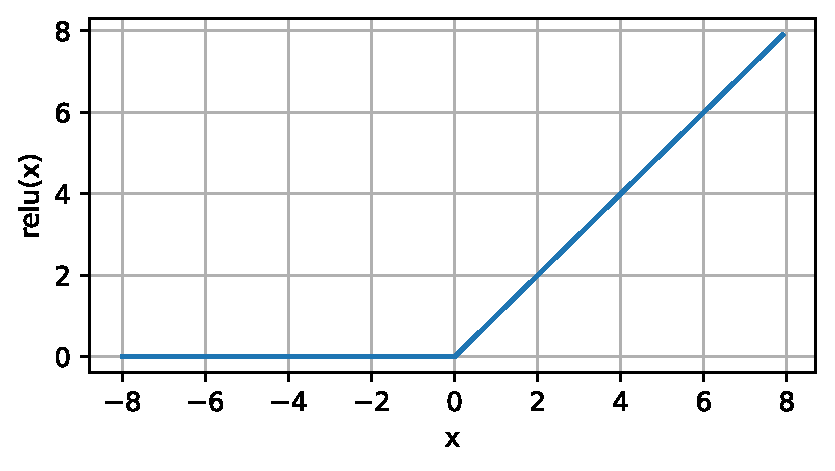
\includegraphics[scale=0.45]{figures/relu}
              
 \end{figure}

\end{frame}
%----------------------------------------------------------------------%
\begin{frame}
\frametitle{Activation Functions}
\begin{itemize}
    \item Parte del atractivo de ReLU tiene que ver con el buen comportamiento de su derivada.
    \begin{itemize}
        \item  Tener en cuenta que la función ReLU no puede diferenciarse cuando la entrada toma un valor exactamente igual a 0. En estos casos, tomamos por defecto la derivada del lado izquierdo y decimos que la derivada es 0 cuando la entrada es 0 (incluso podemos salirse con la nuestra porque la la entrada nunca puede ser realmente cero!)

        \item Esto hace que la optimización se comporte mejor y mitiga el problema de los gradientes que desaparecen.
    \end{itemize}
    
\end{itemize}



  \begin{figure}[H] \centering
            \captionsetup{justification=centering}
              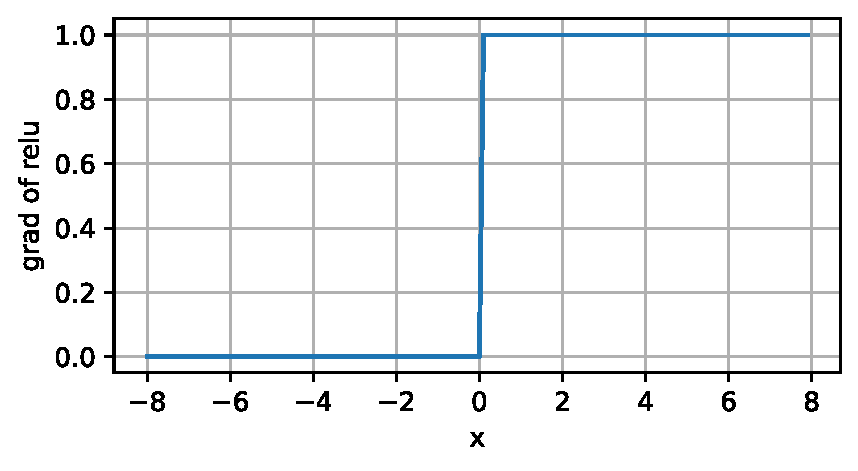
\includegraphics[scale=0.45]{figures/relu_dev}
              
 \end{figure}


\end{frame}
%----------------------------------------------------------------------%
\begin{frame}
\frametitle{Activation Functions}





\begin{itemize}

\item Función sigmoidea

\begin{itemize}



\item La función sigmoidea transforma sus entradas, cuyos valores se encuentran en el dominio $\mathbb{R}$, a salidas que se encuentran en el intervalo (0, 1). 
\item Por esa razón, el sigmoide a menudo se denomina función de aplastamiento: aplasta cualquier entrada en el rango (-inf, inf) a algún valor en el rango (0, 1):

$$\operatorname{sigmoid}(x) = \frac{1}{1 + \exp(-x)}.$$

\item En las primeras redes neuronales, los científicos estaban interesados en modelar neuronas biológicas que se disparan o no. Así, los pioneros de este campo, desde McCulloch y Pitts, los inventores de la neurona artificial, se centraron en las unidades de umbral. Una activación de umbral toma el valor 0 cuando su entrada está por debajo de algún umbral y el valor 1 cuando la entrada excede el umbral.

\item Cuando la atención se centró en el aprendizaje basado en gradientes, la función sigmoidea fue una elección natural porque es una aproximación suave y diferenciable a una unidad de umbral.

    \end{itemize}
\end{itemize}    



\end{frame}
%----------------------------------------------------------------------%
\begin{frame}
\frametitle{Activation Functions}





\begin{itemize}


\item Cuando la atención se centró en el aprendizaje basado en gradientes, la función sigmoidea fue una elección natural porque es una aproximación suave y diferenciable a una unidad de umbral.
\medskip
\item Función sigmoidea



\end{itemize}

  \begin{figure}[H] \centering
            \captionsetup{justification=centering}
              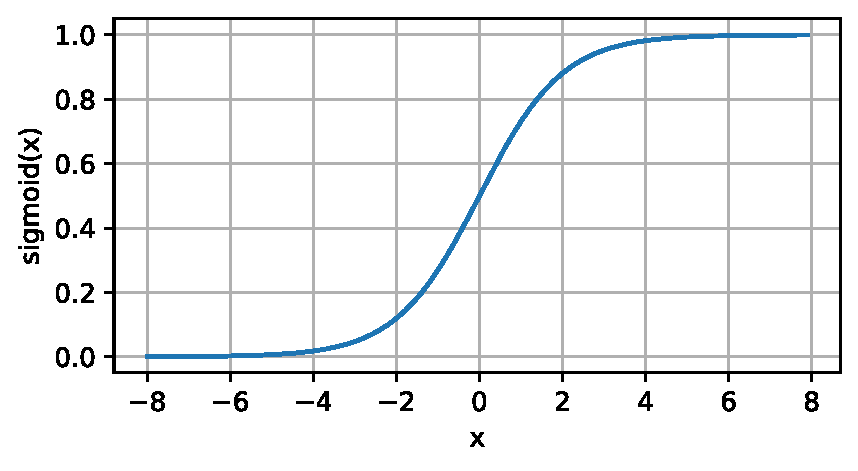
\includegraphics[scale=0.45]{figures/sigmoid}
              
 \end{figure}

\end{frame}

%----------------------------------------------------------------------%
\begin{frame}
\frametitle{Activation Functions}

\begin{itemize}
\item La derivada de la función sigmoidea está dada por la siguiente ecuación:

$$\frac{d}{dx} \operatorname{sigmoid}(x) = \frac{\exp(-x)}{(1 + \exp(-x))^2} = \operatorname{sigmoid}(x)\left(1-\operatorname{sigmoid}(x)\right).$$

\end{itemize}




  \begin{figure}[H] \centering
            \captionsetup{justification=centering}
              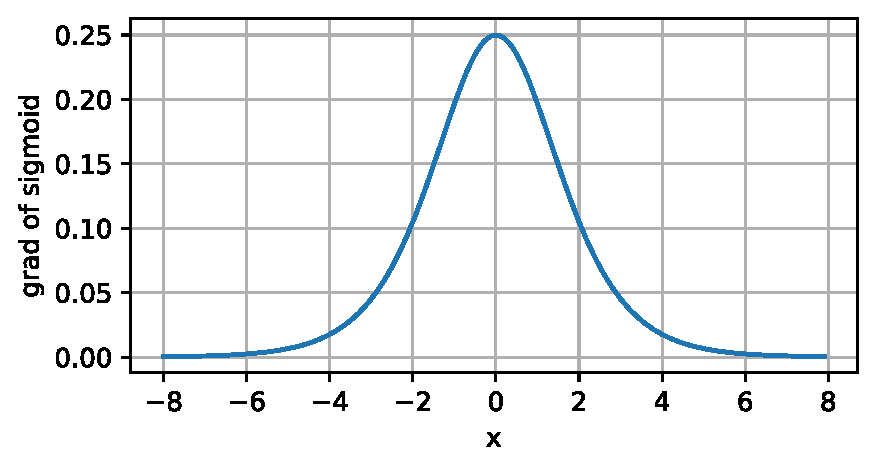
\includegraphics[scale=0.45]{figures/sigmoid_dev}
              
 \end{figure}

\end{frame}

%----------------------------------------------------------------------%
\begin{frame}
\frametitle{Activation Functions}




\begin{itemize}
    
\item Función $Tanh$ 
  \begin{itemize}
        \item Como la función sigmoidea, la función tanh (tangente hiperbóloca) también aplasta sus entradas, transformándolas en elementos en el intervalo entre -1 y 1:

        $$\operatorname{tanh}(x) = \frac{1 - \exp(-2x)}{1 + \exp(-2x)}.$$

        \item Aunque la forma de la función es similar a la de la función sigmoidea, la función $tanh$ exhibe simetría puntual sobre el origen del sistema de coordenadas.
    \end{itemize}
\end{itemize}

  \begin{figure}[H] \centering
            \captionsetup{justification=centering}
              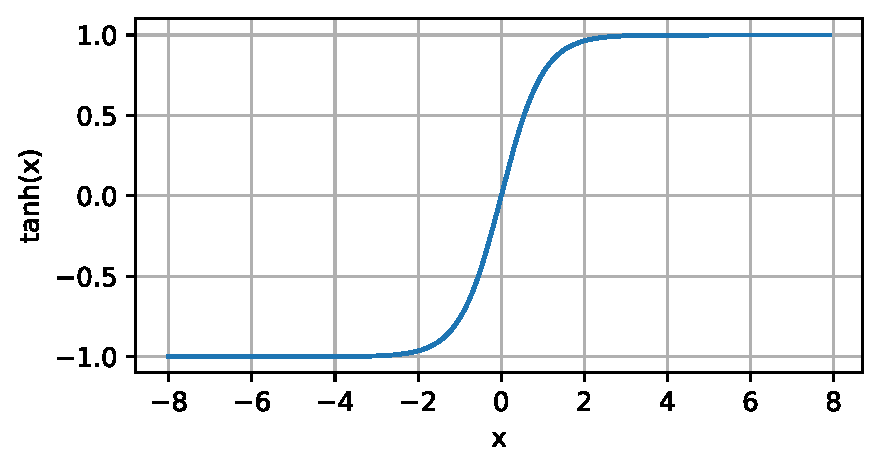
\includegraphics[scale=0.45]{figures/tanh}
              
 \end{figure}

\end{frame}

%----------------------------------------------------------------------%
\begin{frame}
\frametitle{Activation Functions}

\begin{itemize}
\item La derivada de la función $tanh$ es:

$$\frac{d}{dx} \operatorname{tanh}(x) = 1 - \operatorname{tanh}^2(x).$$

\item La derivada de la función $tanh$ está marcada abajo. A medida que la entrada se acerca 0, la derivada de la función $tanh$  se acerca a un máximo de 1. Y como vimos con la función sigmoidea, a medida que la entrada se aleja de 0 en cualquier dirección, la derivada de la función $tanh$ se acerca a 0.
\end{itemize}


  \begin{figure}[H] \centering
            \captionsetup{justification=centering}
              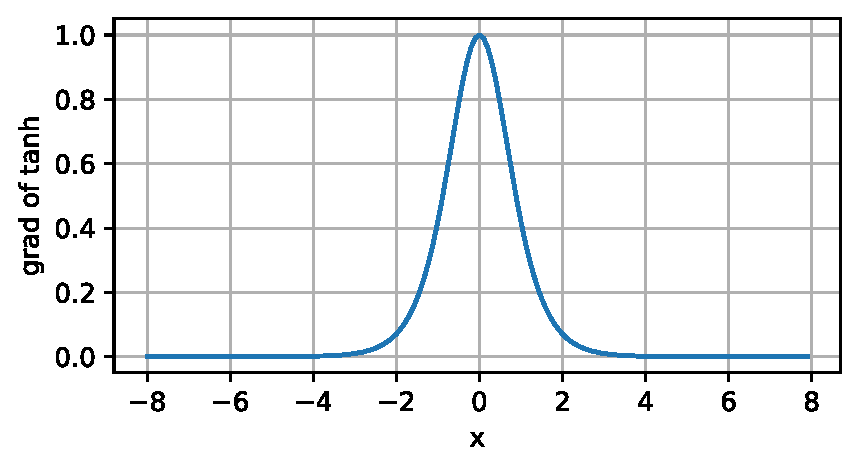
\includegraphics[scale=0.45]{figures/tanh_dev}
              
 \end{figure}



\end{frame}
%----------------------------------------------------------------------%
\begin{frame}
\frametitle{Activation Functions}


\begin{itemize}
\item Otras funciones de activación
\medskip
\begin{itemize}
\item $h=cos(W x+b)$ Goodfellow et all (2016) afirman que en el conjunto de datos MNIST obtuvieron una tasa de error de menos del 1 por ciento
\medskip
\item La función de base radial (RBF): $exp\left( \frac{1}{\sigma^2)}||W-x||^2 \right)$
\medskip
\item Softplus: $log(1+e^x)$
\medskip
\item Hard tanh: $max(-1,min(1,x))$
\medskip
\end{itemize}
\item El diseño de unidades ocultas sigue siendo un área activa de investigación, y quedan muchos tipos de unidades ocultas útiles por descubrir.
\end{itemize}


\end{frame}
%----------------------------------------------------------------------%
\subsubsection{Output Functions}
%----------------------------------------------------------------------%
\begin{frame}
\frametitle{Output Functions}

\begin{itemize}
\item La elección de la función de costo está estrechamente relacionada con la elección de la unidad de salida.
\medskip
\item La mayoría de las veces, simplemente usamos la distancia entre la distribución de datos y la distribución del modelo.
\medskip
\begin{itemize}

    \item Linear $y=W'h +b$ $\rightarrow$  $\mathbb{R}$
    \medskip
    \item Sigmoid (Logistic)$\frac{1}{1 + \exp(-x)}$ $\rightarrow$ clasificación $\{0,1\}$
    \medskip
    \item Softmax $\frac{exp(x)}{\sum exp(x))}$ $\rightarrow$ clasificación de múltiples categorías
\end{itemize}
\end{itemize}

\end{frame}


%----------------------------------------------------------------------%
\subsubsection{Architecture Design}
%----------------------------------------------------------------------%
\begin{frame}
\frametitle{Architecture Design}

\begin{itemize}


\item Otra consideración de diseño clave para las redes neuronales es determinar la arquitectura.

\item La palabra arquitectura se refiere a la estructura general de la red: cuántas unidades debería tener y cómo estas unidades deberían estar conectadas entre sí.

\item En estas arquitecturas basadas en cadenas, las principales consideraciones arquitectónicas son elegir la profundidad de la red y el ancho de cada capa.

\item Un perceptrón multicapa (redes feedforward) con capas ocultas proporcionan un marco de aproximación universal. 
\begin{itemize}
\item El teorema de aproximación universal (Hornik et al., 1989; Cybenko, 1989) establece que una red de retroalimentación con una capa de salida lineal y al menos una capa oculta con cualquier función de activación de "aplastamiento" (como la función de activación sigmoidea logística) puede aproximar cualquier función medible de Borel de un espacio de dimensión finita a otro con cualquier valor distinto de cero cantidad de error, siempre que la red tenga suficiente unidad oculta.

\item La derivada de las redes feedforward también aproximar arbitrariamente bien las derivadas de las funciones (Hornik et al., 1990). 
\end{itemize}



\end{itemize}

\end{frame}
%----------------------------------------------------------------------%
\begin{frame}
\frametitle{Architecture Design}

\begin{itemize}

    \item El teorema de aproximación universal significa que independientemente de la función que estemos tratando de aprender, sabemos que un MLP grande podrá representar esta función.
    \item Sin embargo, no garantiza que el algoritmo de entrenamiento pueda aprender esa función. Incluso si el MLP puede representar la función, el aprendizaje puede fallar por dos razones diferentes.
            \begin{enumerate}
                \item El algoritmo de optimización utilizado
                 para el entrenamiento es posible que no pueda encontrar el valor de los parámetros que corresponde
                 a la función deseada. 
                \item El algoritmo de entrenamiento puede elegir la función incorrecta como resultado de un ajuste excesivo
            \end{enumerate}


    \item Una red de retroalimentación con una sola capa es suficiente para representar cualquier función, pero la capa puede ser inviable grande y puede fallar en aprender y generalizar correctamente.

    \item  En muchas circunstancias, el uso de modelos más profundos puede reducir el número de unidades necesarias para representar la función deseada y puede reducir la cantidad de error de generalización.
    \item  La arquitectura de red ideal para una tarea se debe encontrar a través de la experimentación guiada por el monitoreo del error del conjunto de validación.
\end{itemize}
\end{frame}
% %----------------------------------------------------------------------%
% \subsubsection{Numerical Optimization Issues}
% %----------------------------------------------------------------------%
% \begin{frame}
% \frametitle{Numerical Stability and Initialization}

% \begin{itemize}
% \item Los gradientes que se desvanecen y explotan son problemas comunes en las redes profundas. Es necesario tener mucho cuidado en la inicialización de los parámetros para garantizar que los gradientes y los parámetros permanezcan bien controlados.
% \medskip
% \item Se necesitan heurísticas de inicialización para garantizar que los gradientes iniciales no sean ni demasiado grandes ni demasiado pequeños.
% \medskip
% \item Las funciones de activación de ReLU mitigan el problema del gradiente de desaparición. Esto puede acelerar la convergencia.
% \medskip
% \item La inicialización aleatoria es clave para garantizar que la simetría se rompa antes de la optimización
% \end{itemize}

% \end{frame}
%----------------------------------------------------------------------%

%----------------------------------------------------------------------%
\section{Break}
\begin{frame}
\frametitle{}

\begin{centering}
\huge
\textcolor{andesred}{Volvemos en 15 mins con \texttt{R} }

\end{centering}

\end{frame}
%----------------------------------------------------------------------%
\section{\texttt{R para ML}}
%----------------------------------------------------------------------%
\begin{frame}
\frametitle{R para ML}

\begin{figure}[H] \centering
  \centering
  
\includegraphics[scale=0.35]{../Lecture04/figures/baticomputer_meme.jpg}
  \\
  \tiny photo from \url{https://www.dailydot.com/parsec/batman-1966-labels-tumblr-twitter-vine/}
\end{figure}

\end{frame}


%----------------------------------------------------------------------%
\subsection{Demo}
%----------------------------------------------------------------------%
\begin{frame}[fragile]
\frametitle{Deep Learning: Demo}





\begin{Shaded}
\begin{Highlighting}[]
\KeywordTok{library}\NormalTok{(keras)}
\NormalTok{fashion\_mnist \textless{}{-}}\StringTok{ }\KeywordTok{dataset\_fashion\_mnist}\NormalTok{()}
\end{Highlighting}
\end{Shaded}

  \begin{figure}[H] \centering
            \captionsetup{justification=centering}
              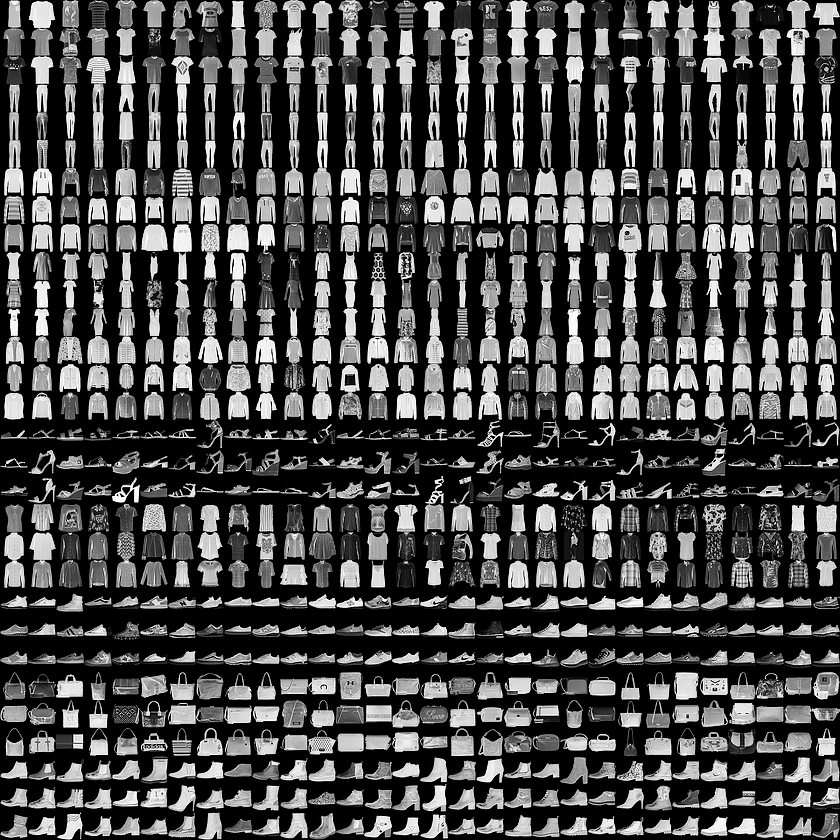
\includegraphics[scale=0.4]{figures/fashion-mnist-sprite}
              
 \end{figure}
\end{frame}
%----------------------------------------------------------------------%
\begin{frame}[fragile]
\frametitle{Deep Learning: Demo}

\begin{Shaded}
\begin{Highlighting}[]


\KeywordTok{c}\NormalTok{(train\_images, train\_labels) }\OperatorTok{\%\textless{}{-}\%}\StringTok{ }\NormalTok{fashion\_mnist}\OperatorTok{$}\NormalTok{train}
\KeywordTok{c}\NormalTok{(test\_images, test\_labels) }\OperatorTok{\%\textless{}{-}\%}\StringTok{ }\NormalTok{fashion\_mnist}\OperatorTok{$}\NormalTok{test}

\NormalTok{class\_names =}\StringTok{ }\KeywordTok{c}\NormalTok{(}\StringTok{\textquotesingle{}T{-}shirt/top\textquotesingle{}}\NormalTok{,}
                \StringTok{\textquotesingle{}Trouser\textquotesingle{}}\NormalTok{,}
                \StringTok{\textquotesingle{}Pullover\textquotesingle{}}\NormalTok{,}
                \StringTok{\textquotesingle{}Dress\textquotesingle{}}\NormalTok{,}
                \StringTok{\textquotesingle{}Coat\textquotesingle{}}\NormalTok{, }
                \StringTok{\textquotesingle{}Sandal\textquotesingle{}}\NormalTok{,}
                \StringTok{\textquotesingle{}Shirt\textquotesingle{}}\NormalTok{,}
                \StringTok{\textquotesingle{}Sneaker\textquotesingle{}}\NormalTok{,}
                \StringTok{\textquotesingle{}Bag\textquotesingle{}}\NormalTok{,}
                \StringTok{\textquotesingle{}Ankle boot\textquotesingle{}}\NormalTok{)}
\end{Highlighting}
\end{Shaded}

\end{frame}
%----------------------------------------------------------------------%
\begin{frame}[fragile]
\frametitle{Deep Learning: Demo}
\begin{scriptsize}

\begin{Shaded}
\begin{Highlighting}[]
\KeywordTok{library}\NormalTok{(tidyr)}
\KeywordTok{library}\NormalTok{(ggplot2)}

\NormalTok{image\_}\DecValTok{1}\NormalTok{ \textless{}{-}}\StringTok{ }\KeywordTok{as.data.frame}\NormalTok{(train\_images[}\DecValTok{1}\NormalTok{, , ])}
\KeywordTok{colnames}\NormalTok{(image\_}\DecValTok{1}\NormalTok{) \textless{}{-}}\StringTok{ }\KeywordTok{seq\_len}\NormalTok{(}\KeywordTok{ncol}\NormalTok{(image\_}\DecValTok{1}\NormalTok{))}
\NormalTok{image\_}\DecValTok{1}\OperatorTok{$}\NormalTok{y \textless{}{-}}\StringTok{ }\KeywordTok{seq\_len}\NormalTok{(}\KeywordTok{nrow}\NormalTok{(image\_}\DecValTok{1}\NormalTok{))}
\NormalTok{image\_}\DecValTok{1}\NormalTok{ \textless{}{-}}\StringTok{ }\KeywordTok{gather}\NormalTok{(image\_}\DecValTok{1}\NormalTok{, }\StringTok{"x"}\NormalTok{, }\StringTok{"value"}\NormalTok{, }\OperatorTok{{-}}\NormalTok{y)}
\NormalTok{image\_}\DecValTok{1}\OperatorTok{$}\NormalTok{x \textless{}{-}}\StringTok{ }\KeywordTok{as.integer}\NormalTok{(image\_}\DecValTok{1}\OperatorTok{$}\NormalTok{x)}

\KeywordTok{ggplot}\NormalTok{(image\_}\DecValTok{1}\NormalTok{, }\KeywordTok{aes}\NormalTok{(}\DataTypeTok{x =}\NormalTok{ x, }\DataTypeTok{y =}\NormalTok{ y, }\DataTypeTok{fill =}\NormalTok{ value)) }\OperatorTok{+}
\StringTok{  }\KeywordTok{geom\_tile}\NormalTok{() }\OperatorTok{+}
\StringTok{  }\KeywordTok{scale\_fill\_gradient}\NormalTok{(}\DataTypeTok{low =} \StringTok{"white"}\NormalTok{, }\DataTypeTok{high =} \StringTok{"black"}\NormalTok{, }\DataTypeTok{na.value =} \OtherTok{NA}\NormalTok{) }\OperatorTok{+}
\StringTok{  }\KeywordTok{scale\_y\_reverse}\NormalTok{() }\OperatorTok{+}
\StringTok{  }\KeywordTok{theme\_minimal}\NormalTok{() }\OperatorTok{+}
\StringTok{  }\KeywordTok{theme}\NormalTok{(}\DataTypeTok{panel.grid =} \KeywordTok{element\_blank}\NormalTok{())   }\OperatorTok{+}
\StringTok{  }\KeywordTok{theme}\NormalTok{(}\DataTypeTok{aspect.ratio =} \DecValTok{1}\NormalTok{) }\OperatorTok{+}
\StringTok{  }\KeywordTok{xlab}\NormalTok{(}\StringTok{""}\NormalTok{) }\OperatorTok{+}
\StringTok{  }\KeywordTok{ylab}\NormalTok{(}\StringTok{""}\NormalTok{)}
\end{Highlighting}
\end{Shaded}

\end{scriptsize}
\end{frame}
%----------------------------------------------------------------------%
\begin{frame}[fragile]
\frametitle{Deep Learning: Demo}
  \begin{figure}[H] \centering
            \captionsetup{justification=centering}
              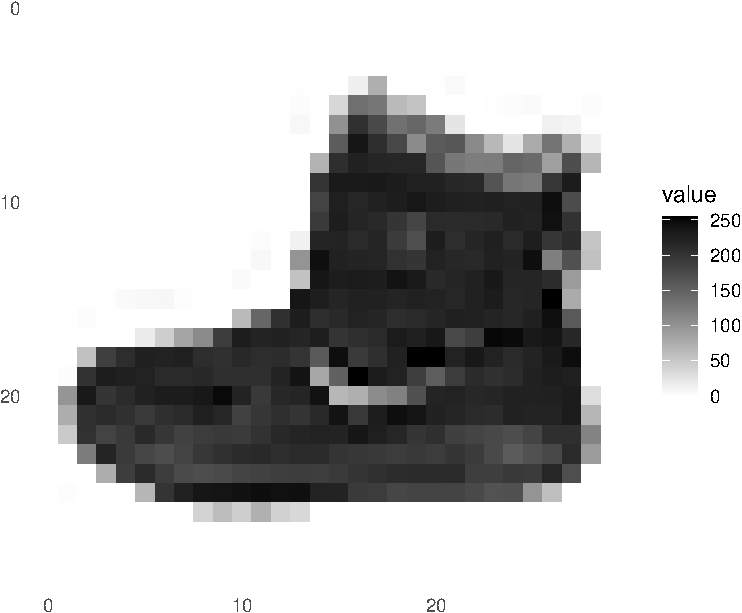
\includegraphics[scale=0.4]{figures/unnamed-chunk-3-1.pdf}
              
 \end{figure}


\end{frame}
%----------------------------------------------------------------------%
\begin{frame}[fragile]
\frametitle{Deep Learning: Demo}

\begin{Shaded}
\begin{Highlighting}[]
\NormalTok{train\_images \textless{}{-}}\StringTok{ }\NormalTok{train\_images }\OperatorTok{/}\StringTok{ }\DecValTok{255}
\NormalTok{test\_images \textless{}{-}}\StringTok{ }\NormalTok{test\_images }\OperatorTok{/}\StringTok{ }\DecValTok{255}
\end{Highlighting}
\end{Shaded}

\begin{Shaded}
\begin{Highlighting}[]
\KeywordTok{par}\NormalTok{(}\DataTypeTok{mfcol=}\KeywordTok{c}\NormalTok{(}\DecValTok{5}\NormalTok{,}\DecValTok{5}\NormalTok{))}
\KeywordTok{par}\NormalTok{(}\DataTypeTok{mar=}\KeywordTok{c}\NormalTok{(}\DecValTok{0}\NormalTok{, }\DecValTok{0}\NormalTok{, }\FloatTok{1.5}\NormalTok{, }\DecValTok{0}\NormalTok{), }\DataTypeTok{xaxs=}\StringTok{\textquotesingle{}i\textquotesingle{}}\NormalTok{, }\DataTypeTok{yaxs=}\StringTok{\textquotesingle{}i\textquotesingle{}}\NormalTok{)}
\ControlFlowTok{for}\NormalTok{ (i }\ControlFlowTok{in} \DecValTok{1}\OperatorTok{:}\DecValTok{25}\NormalTok{) \{ }
\NormalTok{  img \textless{}{-}}\StringTok{ }\NormalTok{train\_images[i, , ]}
\NormalTok{  img \textless{}{-}}\StringTok{ }\KeywordTok{t}\NormalTok{(}\KeywordTok{apply}\NormalTok{(img, }\DecValTok{2}\NormalTok{, rev)) }
  \KeywordTok{image}\NormalTok{(}\DecValTok{1}\OperatorTok{:}\DecValTok{28}\NormalTok{, }\DecValTok{1}\OperatorTok{:}\DecValTok{28}\NormalTok{, img, }\DataTypeTok{col =} \KeywordTok{gray}\NormalTok{((}\DecValTok{0}\OperatorTok{:}\DecValTok{255}\NormalTok{)}\OperatorTok{/}\DecValTok{255}\NormalTok{), }\DataTypeTok{xaxt =} \StringTok{\textquotesingle{}n\textquotesingle{}}\NormalTok{, }\DataTypeTok{yaxt =} \StringTok{\textquotesingle{}n\textquotesingle{}}\NormalTok{,}
        \DataTypeTok{main =} \KeywordTok{paste}\NormalTok{(class\_names[train\_labels[i] }\OperatorTok{+}\StringTok{ }\DecValTok{1}\NormalTok{]))}
\NormalTok{\}}
\end{Highlighting}
\end{Shaded}

\end{frame}
%----------------------------------------------------------------------%
\begin{frame}[fragile]
\frametitle{Deep Learning: Demo}

  \begin{figure}[H] \centering
            \captionsetup{justification=centering}
              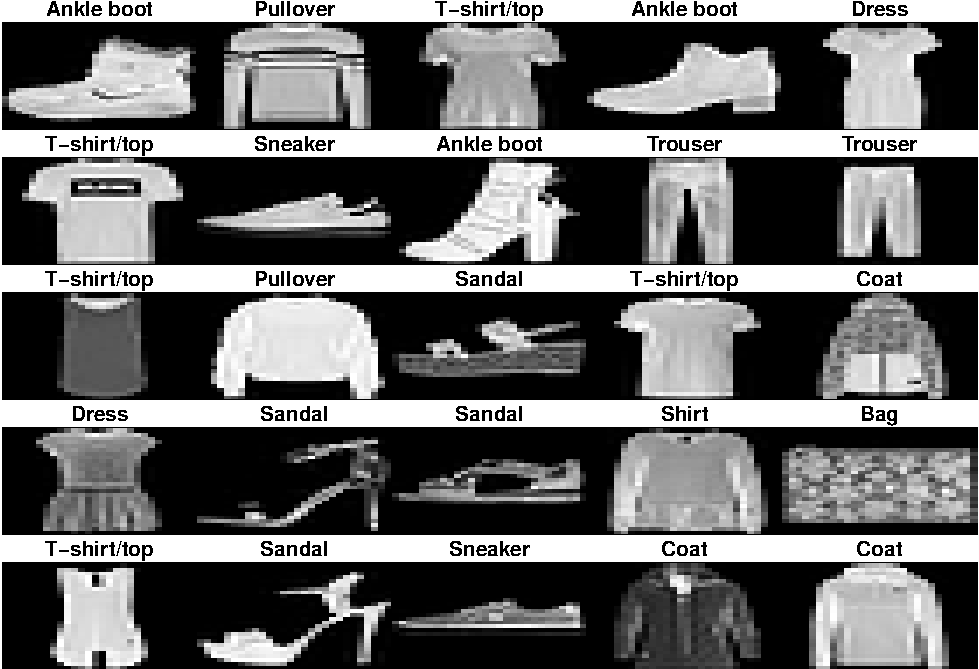
\includegraphics[scale=0.4]{figures/unnamed-chunk-5-1.pdf}
              
 \end{figure}

 \end{frame}
%----------------------------------------------------------------------%
\begin{frame}[fragile]
\frametitle{Deep Learning: Demo}


\begin{Shaded}
\begin{Highlighting}[]
\NormalTok{model \textless{}{-}}\StringTok{ }\KeywordTok{keras\_model\_sequential}\NormalTok{()}
\NormalTok{model }\OperatorTok{\%\textgreater{}\%}
\StringTok{  }\KeywordTok{layer\_flatten}\NormalTok{(}\DataTypeTok{input\_shape =} \KeywordTok{c}\NormalTok{(}\DecValTok{28}\NormalTok{, }\DecValTok{28}\NormalTok{)) }\OperatorTok{\%\textgreater{}\%}
\StringTok{  }\KeywordTok{layer\_dense}\NormalTok{(}\DataTypeTok{units =} \DecValTok{128}\NormalTok{, }\DataTypeTok{activation =} \StringTok{\textquotesingle{}relu\textquotesingle{}}\NormalTok{) }\OperatorTok{\%\textgreater{}\%}
\StringTok{  }\KeywordTok{layer\_dense}\NormalTok{(}\DataTypeTok{units =} \DecValTok{10}\NormalTok{, }\DataTypeTok{activation =} \StringTok{\textquotesingle{}softmax\textquotesingle{}}\NormalTok{)}
\end{Highlighting}
\end{Shaded}

\begin{Shaded}
\begin{Highlighting}[]
\NormalTok{model }\OperatorTok{\%\textgreater{}\%}\StringTok{ }\KeywordTok{compile}\NormalTok{(}
  \DataTypeTok{optimizer =} \StringTok{\textquotesingle{}adam\textquotesingle{}}\NormalTok{, }
  \DataTypeTok{loss =} \StringTok{\textquotesingle{}sparse\_categorical\_crossentropy\textquotesingle{}}\NormalTok{,}
  \DataTypeTok{metrics =} \KeywordTok{c}\NormalTok{(}\StringTok{\textquotesingle{}accuracy\textquotesingle{}}\NormalTok{)}
\NormalTok{)}
\NormalTok{model }\OperatorTok{\%\textgreater{}\%}\StringTok{ }\KeywordTok{fit}\NormalTok{(train\_images, train\_labels, }\DataTypeTok{epochs =} \DecValTok{5}\NormalTok{, }\DataTypeTok{verbose =} \DecValTok{2}\NormalTok{)}
\end{Highlighting}
\end{Shaded}

\end{frame}
%----------------------------------------------------------------------%
\begin{frame}[fragile]
\frametitle{Deep Learning: Demo}
\begin{scriptsize}
\begin{verbatim}
## Epoch 1/5
## 1875/1875 - 2s - loss: 0.5003 - accuracy: 0.8238
## Epoch 2/5
## 1875/1875 - 2s - loss: 0.3782 - accuracy: 0.8643
## Epoch 3/5
## 1875/1875 - 2s - loss: 0.3362 - accuracy: 0.8784
## Epoch 4/5
## 1875/1875 - 2s - loss: 0.3141 - accuracy: 0.8844
## Epoch 5/5
## 1875/1875 - 2s - loss: 0.2934 - accuracy: 0.8922
\end{verbatim}
\end{scriptsize}

\begin{Shaded}
\begin{Highlighting}[]
\NormalTok{score \textless{}{-}}\StringTok{ }\NormalTok{model }\OperatorTok{\%\textgreater{}\%}\StringTok{ }\KeywordTok{evaluate}\NormalTok{(test\_images, test\_labels, }\DataTypeTok{verbose =} \DecValTok{0}\NormalTok{)}

\KeywordTok{cat}\NormalTok{(}\StringTok{\textquotesingle{}Test loss:\textquotesingle{}}\NormalTok{, score[}\DecValTok{1}\NormalTok{], }\StringTok{"}\CharTok{\textbackslash{}n}\StringTok{"}\NormalTok{)}
\end{Highlighting}
\end{Shaded}
\begin{scriptsize}

\begin{verbatim}
## Test loss: 0.3377942

## Test accuracy: 0.8792
\end{verbatim}
\end{scriptsize}
\end{frame}

%----------------------------------------------------------------------%
%----------------------------------------------------------------------%
\end{document}
%----------------------------------------------------------------------%
%----------------------------------------------------------------------%
